% questions.tex —— 2006 年·普通高等学校招生考试·上海卷理科 · 题目内容片段（无答案）
% 由 tools/generate_projects.py 依来源总账自 2006/2006_数学真题_上海理_试题.md 生成，勿手改（改源 MD 后重跑）


\begin{gktip}
\textbf{来源边界}：题面依据本机固定 PDF 第 1–2 页转录。文件 SHA-256 与 source inventory 中固定来源一致。扫描页题签为“2006 普通高等学校招生考试（上海卷理）”，印刷页码为 328–329；这只能确认固定副本的字节和页内可见文字，不能证明 PDF 为考试机构官方原件，也不能确认出版者、版次或扫描来源链。固定扫描件没有答案或解析页。
\end{gktip}

\gkpart{一、填空题}

\begin{question}
\gkti{1}已知集合 $A=\{-1,3,2m-1\}$，集合 $B=\{3,m^2\}$。若 $B\subseteq A$，则实数 $m=$ $\underline{\qquad}$。

\end{question}
\begin{question}
\gkti{2}已知圆 $x^2-4x-4+y^2=0$ 的圆心是点 $P$，则点 $P$ 到直线 $x-y-1=0$ 的距离是 $\underline{\qquad}$。

\end{question}
\begin{question}
\gkti{3}若函数 $f(x)=a^x$（$a>0$，且 $a\ne1$）的反函数的图象过点 $(2,-1)$，则 $a=$ $\underline{\qquad}$。

\end{question}
\begin{question}
\gkti{4}计算：$\displaystyle\lim_{n\to\infty}\frac{\binom n3}{n^3+1}=$ $\underline{\qquad}$。

\end{question}
\begin{question}
\gkti{5}若复数 $z$ 同时满足 $z-\overline z=2i$，$\overline z=iz$（$i$ 为虚数单位），则 $z=$ $\underline{\qquad}$。

\end{question}
\begin{question}
\gkti{6}如果 $\cos\alpha=\dfrac15$，且 $\alpha$ 是第四象限的角，那么 $\cos\left(\alpha+\dfrac\pi2\right)=$ $\underline{\qquad}$。

\end{question}
\begin{question}
\gkti{7}已知椭圆中心在原点，一个焦点为 $F(-2\sqrt3,0)$，且长轴长是短轴长的 2 倍，则该椭圆的标准方程是 $\underline{\qquad}$。

\end{question}
\begin{question}
\gkti{8}在极坐标系中，$O$ 是极点，设点 $A\left(4,\dfrac\pi3\right)$，$B\left(5,-\dfrac{5\pi}6\right)$。则 $\triangle OAB$ 的面积是 $\underline{\qquad}$。

\end{question}
\begin{question}
\gkti{9}两部不同的长篇小说各由第一、二、三、四卷组成，每卷 1 本，共 8 本。将它们任意地排成一排，左边 4 本恰好都属于同一部小说的概率是 $\underline{\qquad}$。（结果用分数表示）

\end{question}
\begin{question}
\gkti{10}如果一条直线与一个平面垂直，那么，称此直线与平面构成一个“正交线面对”。在一个正方体中，由两个顶点确定的直线与含有四个顶点的平面构成的“正交线面对”的个数是 $\underline{\qquad}$。

\end{question}
\begin{question}
\gkti{11}若曲线 $y^2=|x|+1$ 与直线 $y=kx+b$ 没有公共点，则 $k,b$ 分别应满足的条件是 $\underline{\qquad}$。

\end{question}
\begin{question}
\gkti{12}三个同学对问题“关于 $x$ 的不等式
\nopagebreak[4]
\[
x^2+25+|x^3-5x^2|\ge ax
\]
在 $[1,12]$ 上恒成立，求实数 $a$ 的取值范围”提出各自的解题思路。

甲说：“只须不等式左边的最小值不小于右边的最大值。”

乙说：“把不等式变形为左边含变量 $x$ 的函数，右边仅含常数，求函数的最值。”

丙说：“把不等式两边看成关于 $x$ 的函数，作出函数图象。”

参考上述解题思路，你认为他们所讨论的问题的正确结论，即 $a$ 的取值范围是 $\underline{\qquad}$。

\end{question}
\gkpart{二、选择题}

\Needspace{0.4\textheight}
\begin{question}
\gkti{13}如图，在平行四边形 $ABCD$ 中，下列结论中错误的是\mbox{（　　）}。

\begin{gkopts}(1)
\task （A）$\overrightarrow{AB}=\overrightarrow{DC}$
\task （B）$\overrightarrow{AD}+\overrightarrow{AB}=\overrightarrow{AC}$
\task （C）$\overrightarrow{AB}-\overrightarrow{AD}=\overrightarrow{BD}$
\task （D）$\overrightarrow{AD}+\overrightarrow{CB}=\vec 0$
\end{gkopts}
\nopagebreak[4]
\begin{center}% 2006 上海理科卷 Q13；保留原图四顶点的顺序与平行四边形边线。
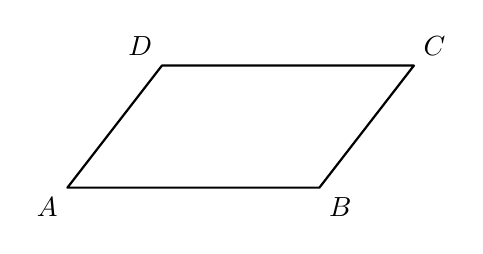
\begin{tikzpicture}[line cap=round,line join=round]
  \coordinate (A) at (0,0);
  \coordinate (B) at (3.2,0);
  \coordinate (C) at (4.4,1.55);
  \coordinate (D) at (1.2,1.55);

  \draw[thick] (A)--(B)--(C)--(D)--cycle;
  \node[below left] at (A) {$A$};
  \node[below right] at (B) {$B$};
  \node[above right] at (C) {$C$};
  \node[above left] at (D) {$D$};
\end{tikzpicture}
\end{center}
\nopagebreak[4]
\end{question}
\begin{question}
\gkti{14}若空间中有四个点，则“这四个点中有三点在同一条直线上”是“这四个点在同一个平面上”的\mbox{（　　）}。

（A）充分非必要条件　（B）必要非充分条件

（C）充分必要条件　（D）既非充分又非必要条件

\end{question}
\begin{question}
\gkti{15}若关于 $x$ 的不等式 $(1+k^2)x\le k^4+4$ 的解集是 $M$，则对任意实常数 $k$，总有\mbox{（　　）}。

\begin{gkopts}(2)
\task （A）$2\in M,\ 0\in M$
\task （B）$2\notin M,\ 0\notin M$
\task （C）$2\in M,\ 0\notin M$
\task （D）$2\notin M,\ 0\in M$
\end{gkopts}

\Needspace{0.4\textheight}
\end{question}
\begin{question}
\gkti{16}如图，平面中两条直线 $l_1$ 和 $l_2$ 相交于点 $O$，对于平面上任意一点 $M$，若 $p,q$ 分别是 $M$ 到直线 $l_1$ 和 $l_2$ 的距离，则称有序非负实数对 $(p,q)$ 是点 $M$ 的“距离坐标”。已知常数 $p\ge0,q\ge0$，给出下列命题：

① 若 $p=q=0$，则“距离坐标”为 $(0,0)$ 的点有且仅有 1 个；

② 若 $pq=0$，且 $p+q\ne0$，则“距离坐标”为 $(p,q)$ 的点有且仅有 2 个；

③ 若 $pq\ne0$，则“距离坐标”为 $(p,q)$ 的点有且仅有 4 个。

上述命题中，正确命题的个数是\mbox{（　　）}。

\begin{gkopts}(4)
\task （A）0
\task （B）1
\task （C）2
\task （D）3
\end{gkopts}
\nopagebreak[4]
\begin{center}% 2006 上海理科卷 Q16；点 M 到两条相交直线的距离用虚线垂线表示。
\begin{tikzpicture}[line cap=round,line join=round]
  \coordinate (O) at (0,0);
  \coordinate (M) at (2.0,1.2);
  \coordinate (P) at (1.6,1.6); % M 到 l_1 的垂足
  \coordinate (Q) at (2.0,0);   % M 到 l_2 的垂足

  \draw[thick] (-2.2,-2.2)--(2.6,2.6) node[above right] {$l_1$};
  \draw[thick] (-2.4,0)--(3.0,0) node[right] {$l_2$};
  \draw[dashed] (M)--(P);
  \draw[dashed] (M)--(Q);
  \draw[thin] (P)--++(-0.14,-0.14)--++(0.14,-0.14)--++(0.14,0.14);
  \draw[thin] (Q)--++(-0.16,0)--++(0,0.16)--++(0.16,0);

  \fill (O) circle[radius=1.2pt];
  \fill (M) circle[radius=1.2pt];
  \node[below left] at (O) {$O$};
  \node[above right] at (M) {$M(p,q)$};
\end{tikzpicture}
\end{center}
\nopagebreak[4]
\end{question}
\gkpart{三、解答题}

\begin{question}
\gkti{17}求函数
\nopagebreak[4]
\[
y=2\cos\left(x+\frac\pi4\right)\cos\left(x-\frac\pi4\right)+\sqrt3\sin2x
\]
的值域和最小正周期。

\Needspace{0.4\textheight}
\end{question}
\begin{question}
\gkti{18}如图，当甲船位于 $A$ 处时获悉，在其正东方向相距 20 海里的 $B$ 处有一艘渔船遇险等待营救。甲船立即前往救援，同时把消息告知在甲船的南偏西 $30^\circ$、相距 10 海里 $C$ 处的乙船，试问乙船应朝北偏东多少度的方向沿直线前往 $B$ 处救援？（角度精确到 $1^\circ$）
\nopagebreak[4]
\begin{center}% 2006 上海理科卷 Q18；按题面方向及距离重绘，图形示意不按比例。
\begin{tikzpicture}[line cap=round,line join=round]
  \coordinate (A) at (0,0);
  \coordinate (B) at (4.3,0);
  \coordinate (C) at (-1.5,-2.598);

  \draw[dashed] (-1.45,0)--(A);
  \draw[dashed] (0,1.75)--(0,-1.45);
  \draw[->] (0.72,1.05)--(0.72,2.05);
  \node[above] at (0.72,2.05) {北};

  \draw[thick] (A)--(B);
  \draw[thick] (A)--(C);
  \draw (0,-0.66) arc[start angle=-90,end angle=-120,radius=0.66];
  \node[above] at (2.15,0) {$20$};
  \node[left] at (-0.92,-1.42) {$10$};
  \node at (-0.28,-0.92) {$30^\circ$};

  \fill (A) circle[radius=1.2pt];
  \fill (B) circle[radius=1.2pt];
  \fill (C) circle[radius=1.2pt];
  \node[above left] at (A) {$A$};
  \node[above right] at (B) {$B$};
  \node[below left] at (C) {$C$};
\end{tikzpicture}
\end{center}
\nopagebreak[4]
\Needspace{0.4\textheight}
\end{question}
\begin{question}
\gkti{19}在四棱锥 $P-ABCD$ 中，底面是边长为 2 的菱形。$\angle DAB=60^\circ$，对角线 $AC$ 与 $BD$ 相交于点 $O$，$PO\perp$ 平面 $ABCD$，$PB$ 与平面 $ABCD$ 所成的角为 $60^\circ$。

（1） 求四棱锥 $P-ABCD$ 的体积；

（2） 若 $E$ 是 $PB$ 的中点，求异面直线 $DE$ 与 $PA$ 所成角的大小。（结果用反三角函数值表示）
\nopagebreak[4]
\begin{center}% 2006 上海理科卷 Q19；四棱锥及底面对角线为矢量示意，不按比例。
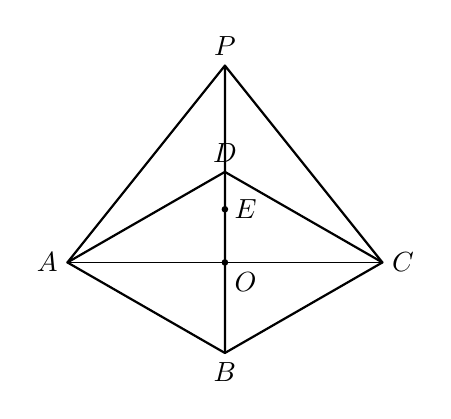
\begin{tikzpicture}[line cap=round,line join=round]
  \coordinate (A) at (-2,0);
  \coordinate (B) at (0,-1.15);
  \coordinate (C) at (2,0);
  \coordinate (D) at (0,1.15);
  \coordinate (O) at (0,0);
  \coordinate (P) at (0,2.5);
  \coordinate (E) at (0,0.675); % PB 的中点

  \draw[thick] (A)--(B)--(C)--(D)--cycle;
  \draw (A)--(C);
  \draw[dashed] (B)--(D);
  \draw[thick] (P)--(A) (P)--(B) (P)--(C) (P)--(D);
  \draw[dashed] (P)--(O);

  \fill (O) circle[radius=1.2pt];
  \fill (E) circle[radius=1.2pt];
  \node[above] at (P) {$P$};
  \node[left] at (A) {$A$};
  \node[below] at (B) {$B$};
  \node[right] at (C) {$C$};
  \node[above] at (D) {$D$};
  \node[below right] at (O) {$O$};
  \node[right] at (E) {$E$};
\end{tikzpicture}
\end{center}
\nopagebreak[4]
\end{question}
\begin{question}
\gkti{20}在平面直角坐标系 $xOy$ 中，直线 $l$ 与抛物线 $y^2=2x$ 相交于 $A,B$ 两点。

（1） 求证：“如果直线 $l$ 过点 $T(3,0)$，那么 $\overrightarrow{OA}\cdot\overrightarrow{OB}=3$”是真命题；

（2） 写出（1）中命题的逆命题，判断它是真命题还是假命题，并说明理由。

\end{question}
\begin{question}
\gkti{21}已知有穷数列 $\{a_n\}$ 共有 $2k$ 项（整数 $k\ge2$），首项 $a_1=2$。设该数列的前 $n$ 项和为 $S_n$，且
\nopagebreak[4]
\[
a_{n+1}=(a-1)S_n+2\quad(n=1,2,\ldots,2k-1),
\]
其中常数 $a>1$。

（1） 求证：数列 $\{a_n\}$ 是等比数列；

\Needspace{5\baselineskip}
（2） 若 $a=2^{\frac{2}{2k-1}}$，数列 $\{b_n\}$ 满足
\nopagebreak[4]
\[
b_n=\frac1n\log_2(a_1a_2\cdots a_n)\quad(n=1,2,\ldots,2k),
\]
求数列 $\{b_n\}$ 的通项公式；

\Needspace{5\baselineskip}
（3） 若（2）中的数列 $\{b_n\}$ 满足不等式
\nopagebreak[4]
\[
\left|b_1-\frac32\right|+\left|b_2-\frac32\right|+\cdots+
\left|b_{2k}-\frac32\right|\le4,
\]
求 $k$ 的值。

\end{question}
\begin{question}
\gkti{22}已知函数 $y=x+\dfrac ax$ 有如下性质：如果常数 $a>0$，那么该函数在 $(0,\sqrt a]$ 上是减函数，在 $[\sqrt a,+\infty)$ 上是增函数。

（1） 如果函数 $y=x+\dfrac{2b}{x}$（$x>0$）的值域为 $[6,+\infty)$，求 $b$ 的值；

（2） 研究函数 $y=x^2+\dfrac c{x^2}$（常数 $c>0$）在定义域内的单调性，并说明理由；

\Needspace{5\baselineskip}
（3） 对函数 $y=x+\dfrac ax$ 和 $y=x^2+\dfrac a{x^2}$（常数 $a>0$）作出推广，使它们都是你所推广的函数的特例。研究推广后的函数的单调性（只须写出结论，不必证明），并求函数
\nopagebreak[4]
\[
F(x)=\left(x^2+\frac1x\right)^n+
\left(\frac1{x^2}+x\right)^n
\]
（$n$ 是正整数）在区间 $\left[\dfrac12,2\right]$ 上的最大值和最小值。（可利用你的研究结论）

\end{question}